\chapter{Experiment}

\section{Dataset}

\subsection{Stanford Sentiment Treebank}
In this thesis, we use Standford Sentiment Treebank (SST) dataset \cite{socher2013recursive}. Standford Sentiment Treebank contains 11,855 sentences. Each data sentence consist of fined-grain sentiment labeled phrases in constituency parse tree structure (see \textbf{Figure \ref{fig:sst}}). There are total 215,154 phrases in whole dataset.
The dataset was splitted into train/dev/test contain 8544/1101/2210 sentences each for training and evaluation models. After remove neutral sentiment sentences, there are 6920/872/1821 sentences remained in train/dev/test set.

SST dataset are publicly available online \footnote{https://nlp.stanford.edu/sentiment/index.html}.

\subsubsection{Preprocess}
We use preprocess source code from \cite{socher2013recursive} implementation \footnote{\url{https://github.com/stanfordnlp/treelstm}} to preprocess SST.



\subsection{Amazon Movies Review}
We get Amazon Movies and TV reviews (4,607,047 reviews) and Amazon Book reviews (22,507,155 reviews) \cite{he2016ups}. Listing \ref{lst:amzrevie} is sample of one book review.

%TODO: change to book example
\begin{lstlisting}[caption={Amazon reviews sample},label={lst:amzreview}]
	{
	  "reviewerID": "A2SUAM1J3GNN3B",
	  "asin": "0000013714",
	  "reviewerName": "J. McDonald",
	  "helpful": [2, 3],
	  "reviewText": "I bought this for my husband who plays the piano.  He is having a wonderful time playing these old hymns.  The music  is at times hard to read because we think the book was published for singing from more than playing from.  Great purchase though!",
	  "overall": 5.0,
	  "summary": "Heavenly Highway Hymns",
	  "unixReviewTime": 1252800000,
	  "reviewTime": "09 13, 2009"
	}
\end{lstlisting}

We extract reviewText and overall from review dataset. We use overall as sentiment score for reviews, with 5 is very positive and 0 is very negative.



% how to preprocess amazon movies reviews
We get Amazon Movies and TV reviews (4,607,047 reviews) and Amazon Book reviews (22,507,155 reviews) \cite{he2016ups} as our training dataset for our word embedding layer. First, we join both dataset and shuffle. Then, we group review of same produce together. Finally, for each product, we sort reviews based on score. Hence, neighbor reviews have similar sentiment and talk about same product, except at the boundary of two produces. We also create one version of dataset which we only shuffle the data without group or sort for comparision. We train our word representation from Amazon dataset using Glove \cite{pennington2014glove} on 15 iteration with windows size of 20.


\begin{figure}[H]
	\begin{minipage}{\textwidth}
		\centering
		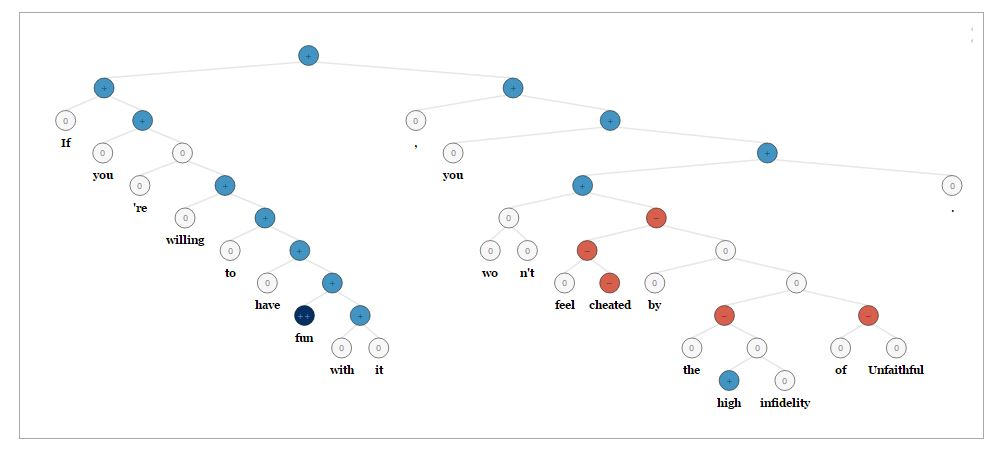
\includegraphics[width=0.9\linewidth]{figure/sst}
		\caption[A parsed sentence in SST]{A parsed sentence in SST \footnote{Render by Pytreebank \url{https://github.com/JonathanRaiman/pytreebank}}}
		\label{fig:sst}
	\end{minipage}
\end{figure}



\section{Embedding}
We run experiment on variety of pre-trained word representation.

\section{title}

% Please add the following required packages to your document preamble:
% \usepackage{booktabs}
% Please add the following required packages to your document preamble:
% \usepackage{booktabs}
\begin{table}[]
	\centering
	\caption{My caption}
	\label{my-label}
	\begin{tabular}{@{}lll@{}}
		\toprule
		& Constituency Tree-LSTM & LSTM \\ \midrule
		Glove 42B             &                        &      \\
		Glove 840B            &                        &      \\
		Glove (Amazon)        &  88.45           &      \\
		Glove (Amazon Sorted) &  88.85           &      \\
		Paragram-Phrase XXL   &                        &      \\
		SSWEu                 &                        &      \\ \bottomrule
	\end{tabular}
\end{table}
